\documentclass[12pt]{article}
\usepackage{amsmath}
\usepackage{amsfonts}
\usepackage{hyperref}
\usepackage{textcomp}
\usepackage{parskip}
\usepackage{graphicx}
\graphicspath{ {images/} }
\hypersetup{
    colorlinks,
    citecolor=black,
    filecolor=black,
    linkcolor=black,
    urlcolor=black
}
\author{Andrija Milovac, Roko Burilo}
\title{Dave The Computer Guy}
\date{22.4.2022}
\begin{document}
\maketitle
\tableofcontents
\section{Product vision}
\subsection{Simple explanation}
Dave The Computer Guy is a web game with the goal of teaching you how to build a computer from scratch out of logic gates step by step.
\subsection{Story intro}

You are in control of Dave, a fresh computer science graduate who has worked as a software developer throughout his education.
After he graduated, he applied for a job at a local electronics manufacturer called "Electro Nick's" because he wanted to 
improve his knowledge of the hardware side of computers.

He got the job and now works in the company's office with his assigned mentor and senior hardware developer John Dodi and their boss Dexter Crawford.

Dave's job consists of syncing with his boss about the work that needs to be done and doing the required work which is mostly
creating new electronic components.

Whenever Dave gets stuck on a task or has no idea where to even start he can always ask John Dodi for help as he is a senior developer with
decades of experience and wisdom.

Dave is really motivated and decided to take on a side project in which he will make his very own computer at home by using the knowledge 
he acquires at work.
\subsection{Graphics}

The game will use WebGL to display its graphics.\\
The graphics are 3D and voxel models will be used.\\
An isometric camera will be used to view the scenes.\\
There will be 3 main scenes in which the player will play:\\
\begin{enumerate}
    \item The office - Dave's workplace
          \begin{center}
              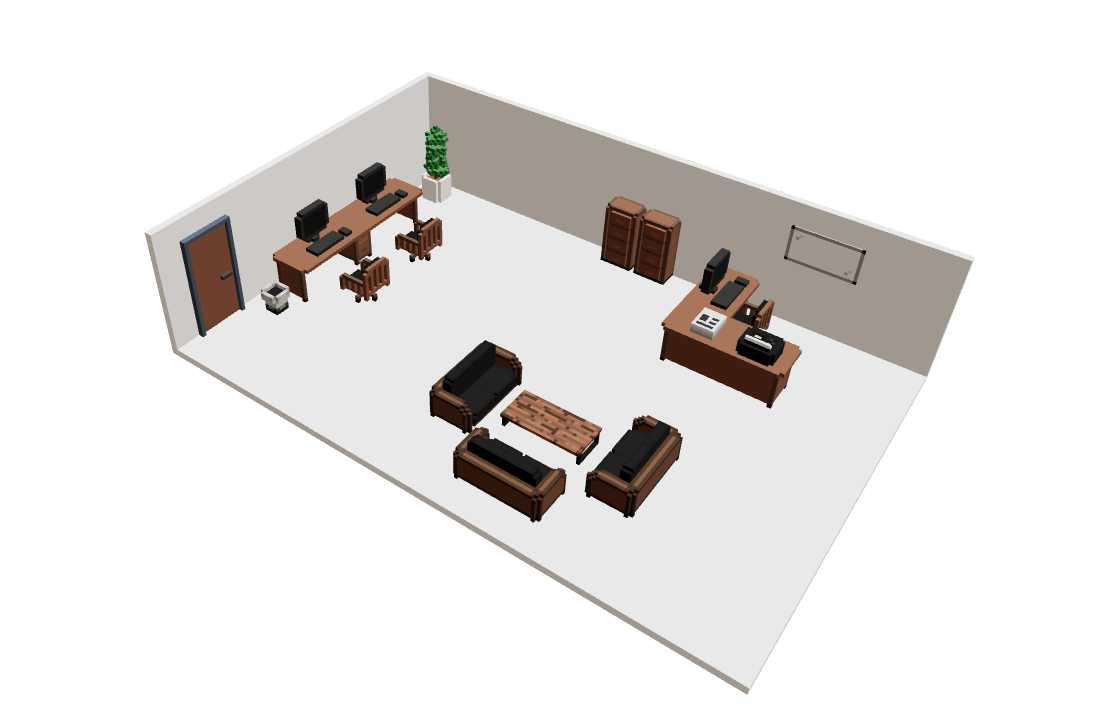
\includegraphics[width=5cm, height=4cm]{office.png}
          \end{center}
          \pagebreak
    \item Home - Dave's home where he spends time creating his own circuits and finally his own computer.
          \begin{center}
              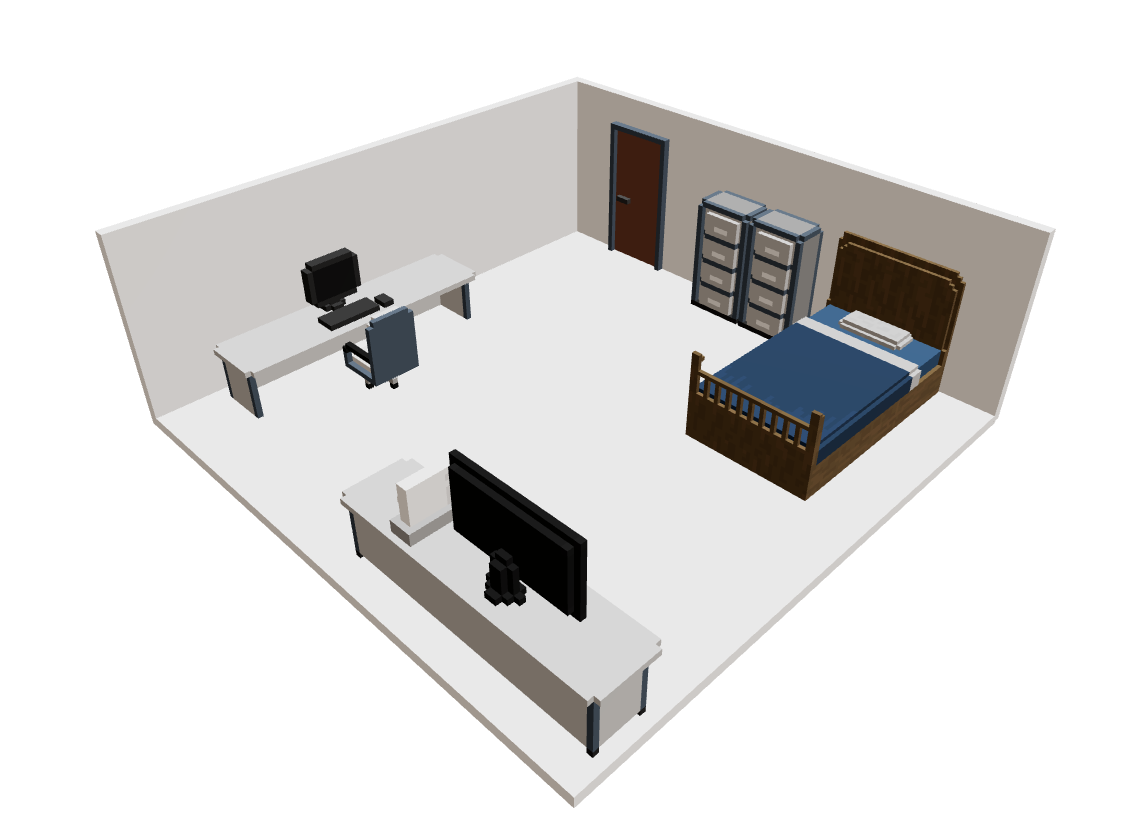
\includegraphics[width=5cm, height=4cm]{home.png}
          \end{center}
    \item Electronics shop - Dave buys circuit parts here from a salesman named Adem Shady
          \begin{center}
              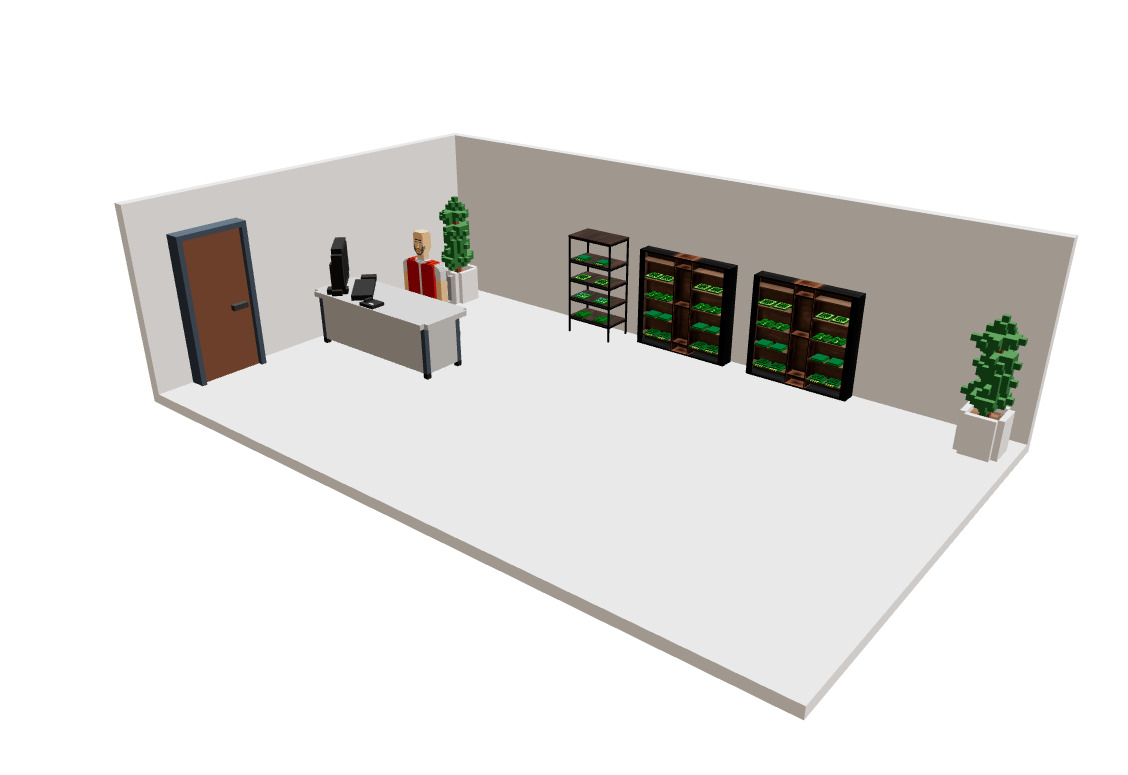
\includegraphics[width=5cm, height=4cm]{shop.jpeg}
          \end{center}
\end{enumerate}

Each of the mentioned 3D scenes will contain clickable elements that will open additional UI elements where the gameplay will actually happen 
like for example the circuit editor window.
\pagebreak

\subsection{Player models}
There are 3 NPC models and 1 player model.

The NPCs are:

\begin{enumerate}
    \item Dexter Crawford - the boss
    \item John Dodi - the senior engineer
    \item Adam Shady - the shop clerk
\end{enumerate}

The models can be viewed down below:

\begin{enumerate}
    \item Dexter Crawford - the boss
          \begin{center}
              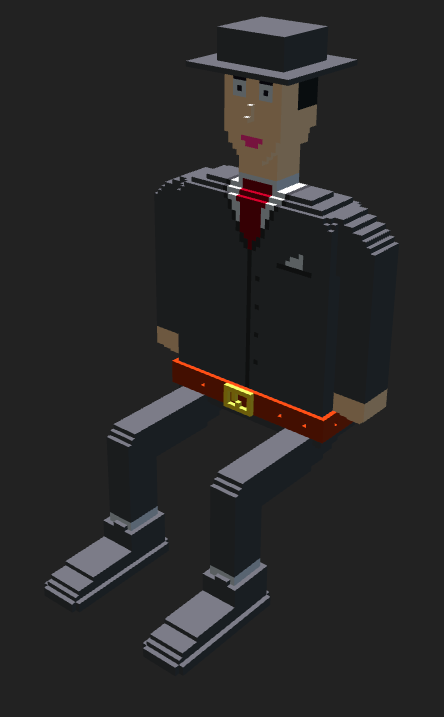
\includegraphics[width=5cm, height=4cm]{boss.png}
          \end{center}
    \item John Dodi - the senior engineer
          \begin{center}
              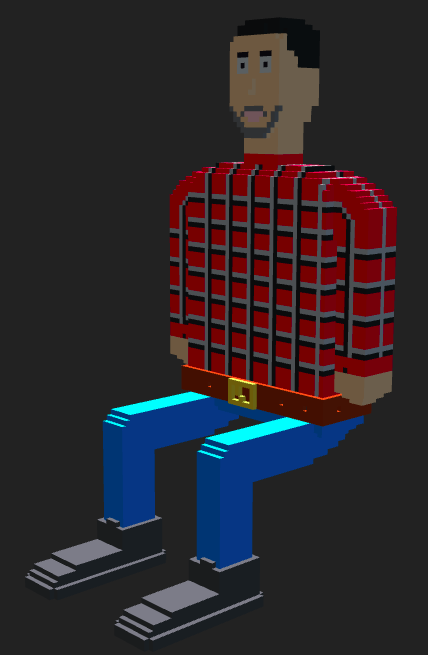
\includegraphics[width=5cm, height=4cm]{john-dodi.png}
          \end{center}
          \pagebreak
    \item Adam Shady - the shop clerk
          \begin{center}
              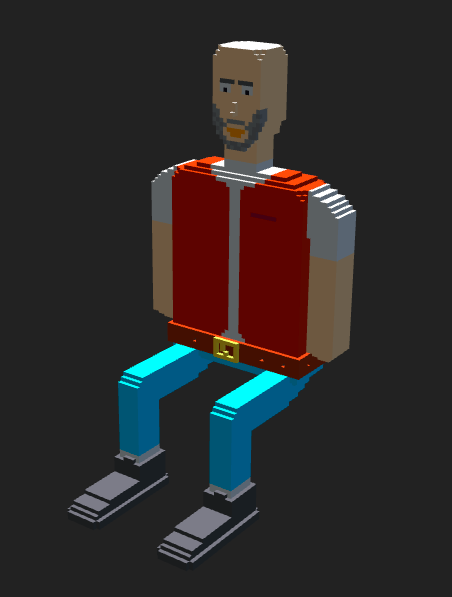
\includegraphics[width=5cm, height=4cm]{clerk.png}
          \end{center}
    \item Dave - the player
          \begin{center}
              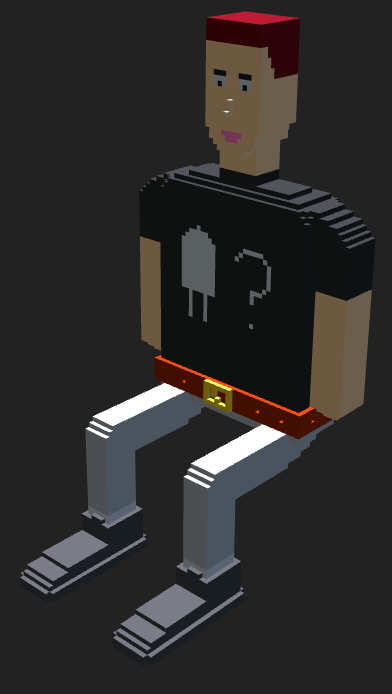
\includegraphics[width=5cm, height=4cm]{player.png}
          \end{center}
\end{enumerate}

\subsection{Gameplay}
The goal of the game is to build your own computer at home.\\
The main gameplay will take part in the circuit editor window which you will use to create new components/circuits 
and analyse existing circuits/components.
The game will follow a linear path which is of the following form:
\begin{enumerate}
    \item Get an assignment from your boss.
    \item Solve the assignment. (this includes producing various components and buying the necessary parts to make the components)
    \item Get paid for solving the assignment and unlock new components.
    \item Use the knowledge you've acquired to advance your computer during your free-time at home.
    \pagebreak
    \item Once you progressed and unlocked every type of component you will get the final mission of building a computer.
    \item Once you build a computer that satisfies the given conditions (checked via tests made by the developers) you have officially completed the main story of the game.
    \item The game does not end once you build the computer, you can still work at your job and earn resources and make new circuits and components.
\end{enumerate}



\section{Product market}
The audience for this product are people in love with computers as well as college students.\\
The product could be used by universities to teach computer architecture in a fun, engaging and rewarding way.\\
The game will have ads with the option of paying a one time fee to remove them for your account.
\section{Product implementation}

The core simulator will be written in Rust (compiled into WASM).
The simulator will be event driven and you will be able to observe signal values over time.

The frontend of this application will be made using the following technologies:
\begin{itemize}
    \item Svelte (Sveltekit) as the frontend framework
    \item Threlte (Three.js) as the webGL framework (library)
    \item TailwindCSS for styling
\end{itemize}
The backend of this application will be made using the following technologies:
\begin{itemize}
    \item Vert.x on the backend
    \item MongoDB as the database
\end{itemize}

\textit{DISCLAIMER: Anything in the product implementation is subject to change.}
\end{document}
